\chapter{Servicios básicos: UDP y TCP}\label{chap:1}
\section{Programación de red: UDP}

En esta sesión se estudia el desarrollo de servicios UDP.
A lo largo de esta sesión, se utilizan 2 programas: Un cliente y un servidor.
Los distintos ejercicios muestran mejoras a realizar en ambos programas
para fortalecer la robustez de la comunicación.

Ya que muchos ejercicios son parecidos en el código y salida,
puede que en algunos casos sólo se haga una mención a la mejora implementada.

\subsection{Módulos de ayuda}
Para esta práctica, se desarrollan módulos de Python que faciliten las tareas básicas,
como lecturas de hosts y puertos por argumentos: \\
\begin{minipage}{\linewidth}
	\centering
	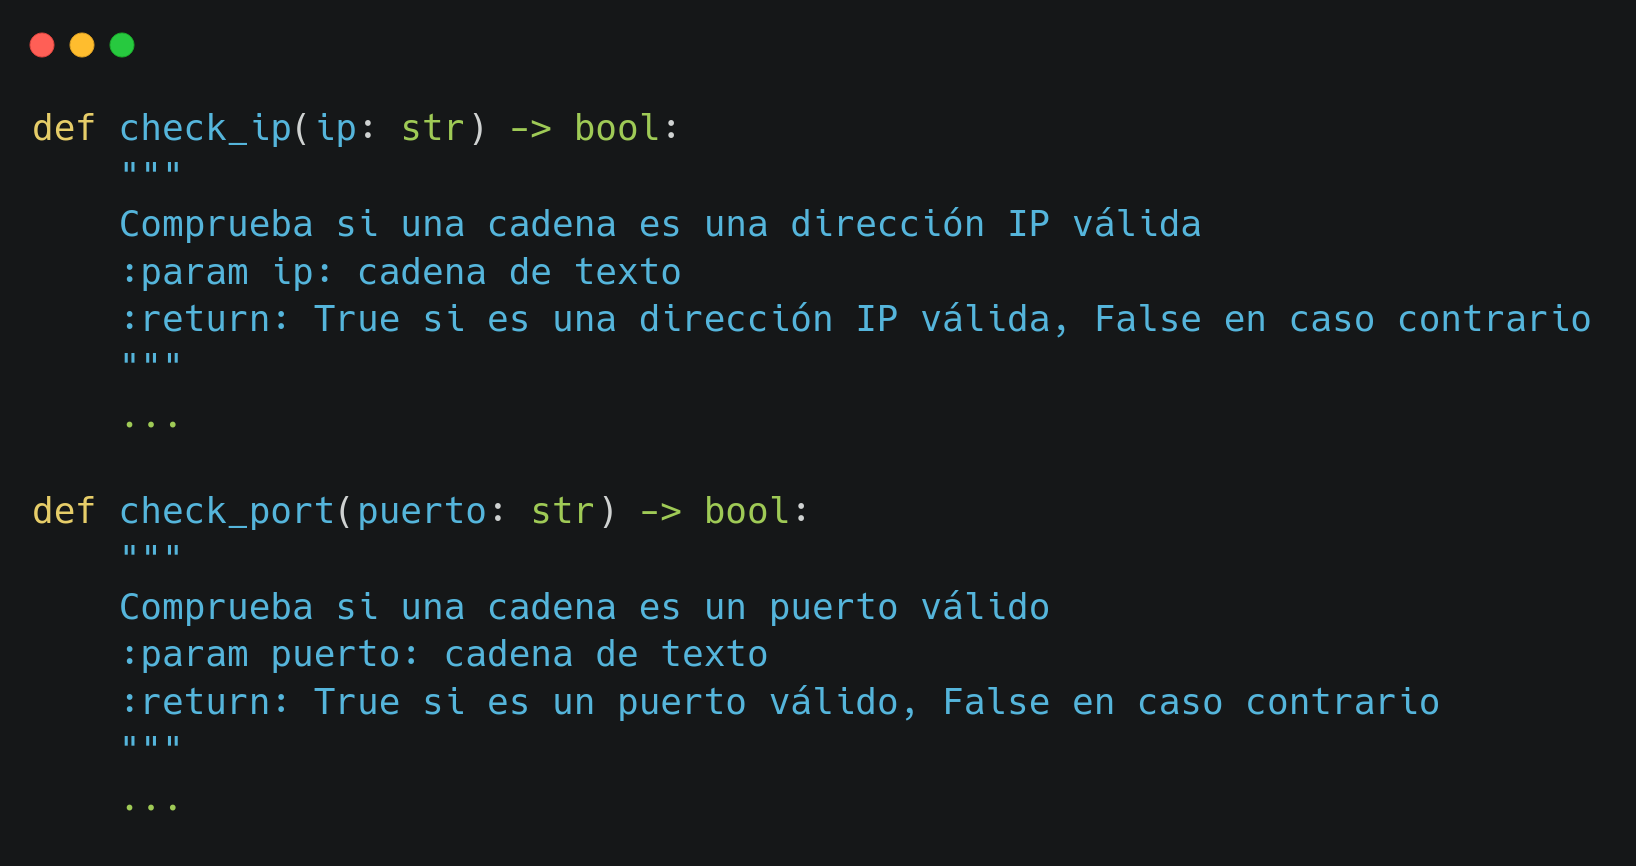
\includegraphics[width=1\textwidth]{1/code1.png}
	\captionof{figure}{Estructura del módulo de ayuda ``ips.py''}\label{fig:1/code1}
\end{minipage}
\\
\begin{minipage}{\linewidth}
	\centering
	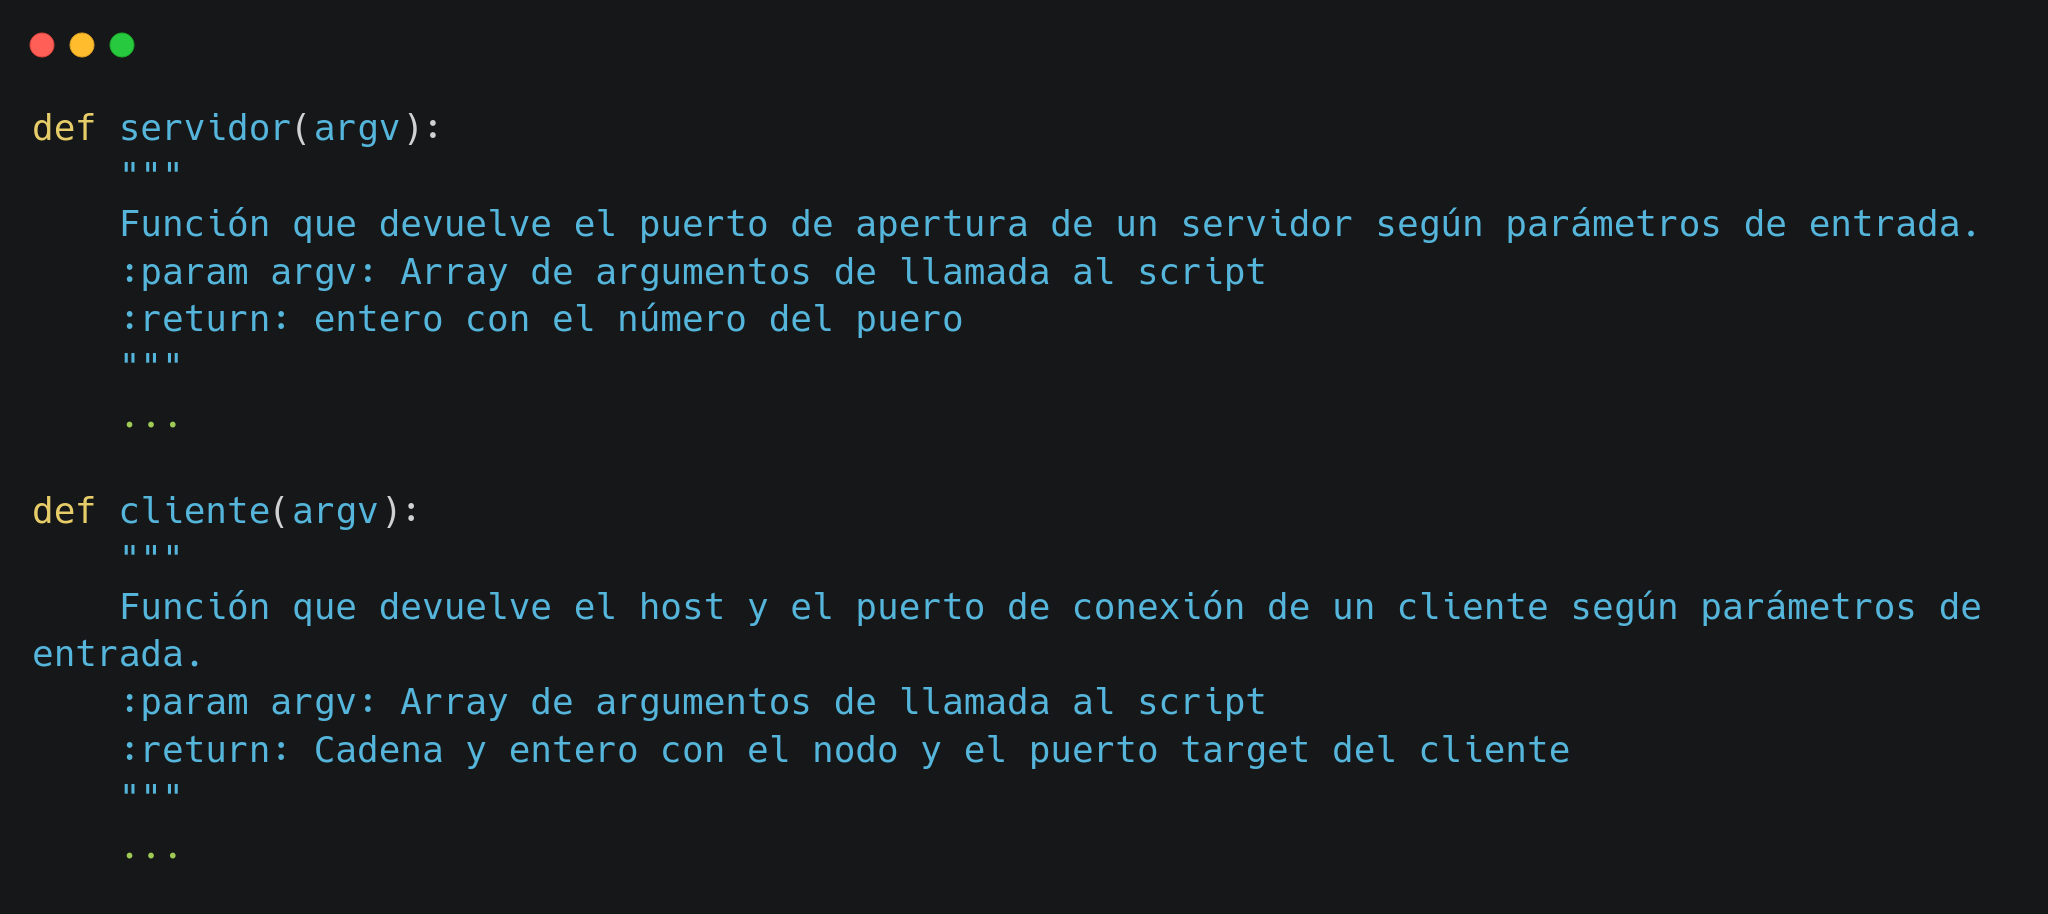
\includegraphics[width=1\textwidth]{1/code2.png}
	\captionof{figure}{Estructura del módulo de ayuda ``ips\_argv.py''}\label{fig:1/code2}
\end{minipage}

\subsection{UDP}

Inicialmente se desarollan un servidor y un cliente simples.
El servidor se encuentra a la espera de mensajes de clientes
y el cliente se conecta a un servidor (cuya IP es conocida de antemano)
al que le envía un mensaje.
Cuando el servidor recibe un mensaje, lo imprime por pantalla.

\begin{minipage}{\linewidth}
	\centering
	\includegraphics[width=\textwidth]{1/UDP/1.png}
	\captionof{figure}{Cliente y Servidor Simples}\label{fig:1/1}
\end{minipage}

A continuación se modifica el código del servidor para que
simule la pérdida de algunos mensajes enviados por los clientes.
Para ello, se utiliza un número aleatorio de forma que se pierdan
el 50\percentsign de los paquetes.

\begin{minipage}{\linewidth}
	\centering
	\includegraphics[width=\textwidth]{1/UDP/2.png}
	\captionof{figure}{El servidor simula pérdidas}\label{fig:1/2}
\end{minipage}

El cliente es modificado de forma que al enviar un mensaje,
lo etiquete con un índice.
El índice es simplemente un contador que se incrementa en uno
por cada mensaje que se envía.

Se realiza una modificación en el servidor de forma que envíe
un OK al cliente cuando el mensaje no se ha perdido
(el 50\percentsign de las veces).

El cliente ahora espera un mensaje con OK del servidor.
Sin embargo, no puede quedarse esperando constantemente ya que esto
dejaría al cliente atascado si se pierde el paquete.
Se implementa un timeout para que esto no suceda.

A continuación, el cliente es modificado para que si el timeout caduca
se intente reenviar el mensaje.
El timeout se verá incrementado con cada reintento para combatir la posible
congestión de la red hasta un máximo de 2 segundos, cuando el cliente
se dará por vencido.

\begin{minipage}{\linewidth}
	\centering
	\includegraphics[width=\textwidth]{1/UDP/3.png}
	\captionof{figure}{El cliente reintenta el envío si no recibe un OK del servidor}\label{fig:1/3}
\end{minipage}

\subsection{Broadcast en UDP}

Se utilizan el cliente y servidor anteriores para implementar un servicio nuevo "HOLA".
Un cliente que quiera utilizar este servicio deberá conectarse a un servidor que implemente
el servicio HOLA.
No obstante, en este caso se tiene en cuenta que puede que el cliente no conozca la dirección
IP del servidor (o servidores) que implementan este servicio.
Para resolver este problema, se utilizan mensajes en broadcast.
Un cliente que quiera interactuar con el servicio deberá enviar un mensaje a broadcast
preguntando por servidores que implementen HOLA.
Si un servidor que imlementa HOLA recibe este mensaje broadcast, deberá responder al cliente.
El cliente, al recibir la respuesta del servidor, conoce su dirección IP y podrá utilizar su servicio.
En caso de recibir múltiples respuestas de varios servidores
el cliente utilizará al primer servidor que responda.

\begin{notebox}
    En este apartado no se muestran capturas de pantalla de la ejecución.
    Esto se debe a que este mismo ejercicio se ejecuta utilizando Docker en el siguiente apartado.
    Ver el siguiente apartado para las capturas de pantalla de este ejercicio.
\end{notebox}

\subsection{Despliegue con Docker}

Este apartado consiste en migrar el servicio HOLA creado anteriormente a un contenedor Docker.
Se indica que creemos 3 contenedores Docker de servidores que implementan HOLA
y un contenedor de un cliente en busca de un servidor que implemente HOLA.

\begin{minipage}{\linewidth}
	\centering
	\includegraphics[width=\textwidth]{1/UDP/4.png}
	\captionof{figure}{Servicio HOLA}\label{fig:1/2}
\end{minipage}

\section{Programación de red: TCP}

Esta sesión trata el protocolo TCP.
En particular, se centra en estudiar las distintas estrategias a la hora
de conocer el fin del mensaje.

\subsection{Módulos de ayuda}
Se reutilizan los módulos de la sesión anterior (\ref{fig:1/code1}~y~\ref{fig:1/code2}) para
realizar todos los ejercicios. Además, para los ejercicios ``oche'' se reutiliza el código
usando otro módulo nuevo: \\
\begin{minipage}{\linewidth}
	\centering
	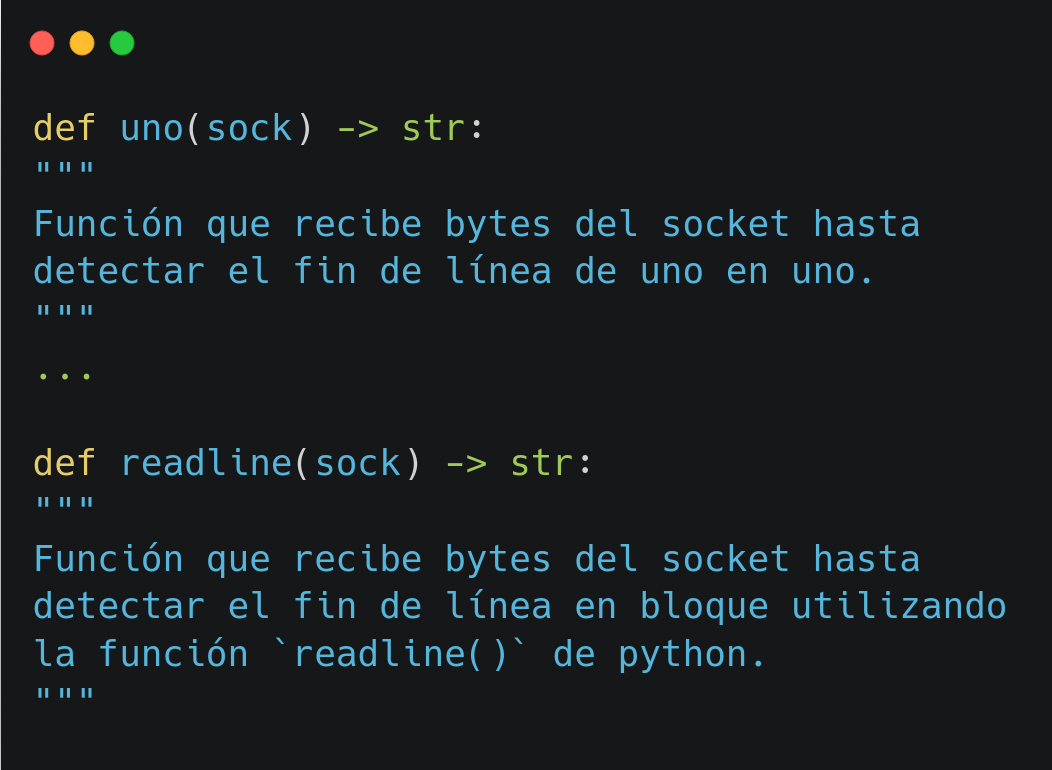
\includegraphics[width=1\textwidth]{1/code3.png}
	\captionof{figure}{Estructura del módulo de ayuda ``recibir\_mensaje.py''}\label{fig:1/code3}
\end{minipage}

\subsection{Tamaño Prefijado}

Inicialmente, se fija un tamaño de 5 bytes por mensaje.
Se escriben un cliente y servidor que trabajan con mensajes de longitud 5 bytes.

\begin{minipage}{\linewidth}
	\centering
	\includegraphics[width=\textwidth]{1/TCP/1.png}
	\captionof{figure}{V1}\label{fig:1/4}
\end{minipage}

En una segunda versión, se utiliza una función que recibe todos los bytes
independientemente de si llegan seguidos o no.

A efectos de la salida, no hay cambios a menos que las condiciones de la red
impliquen un cambio en el envío de los mensajes.

\begin{minipage}{\linewidth}
	\centering
	\includegraphics[width=\textwidth]{1/TCP/2.png}
	\captionof{figure}{V2}\label{fig:1/5}
\end{minipage}

Si modificamos el número de bytes en los mensajes,
curiosamente se vuelven a leer desde el principio una vez terminados.

Esto es, si se envía el mensaje \verb#ABCD# y el código indica que se deben leer
5 bytes, se leerá \verb#ABCDA#.

Esto sucede tanto en la primera como en la segunda versión del servidor.

\begin{minipage}{\linewidth}
	\centering
	\includegraphics[width=\textwidth]{1/TCP/3.png}
	\captionof{figure}{V2}\label{fig:1/5}
\end{minipage}

\subsection{Marca de Fin de Mensaje}

Los siguientes clientes y servidores utilizan un retorno de carro
para indicar el fin de mensaje.

El siguiente ejemplo consiste de un cliente que envía un mensaje
con \verb#\r\n# al final
y un servidor que al recibir dicho mensaje lo retorna dado la vuelta.

\begin{minipage}{\linewidth}
	\centering
	\includegraphics[width=\textwidth]{1/TCP/4.png}
	\captionof{figure}{Oche Simplista}\label{fig:1/6}
\end{minipage}

A continuación, se modifica el cliente para que envie 3 mensajes
seguidos y posteriormente espere 3 mensajes de vuelta.

Se muestra una imagen con la salida de estos programas:

\begin{minipage}{\linewidth}
	\centering
	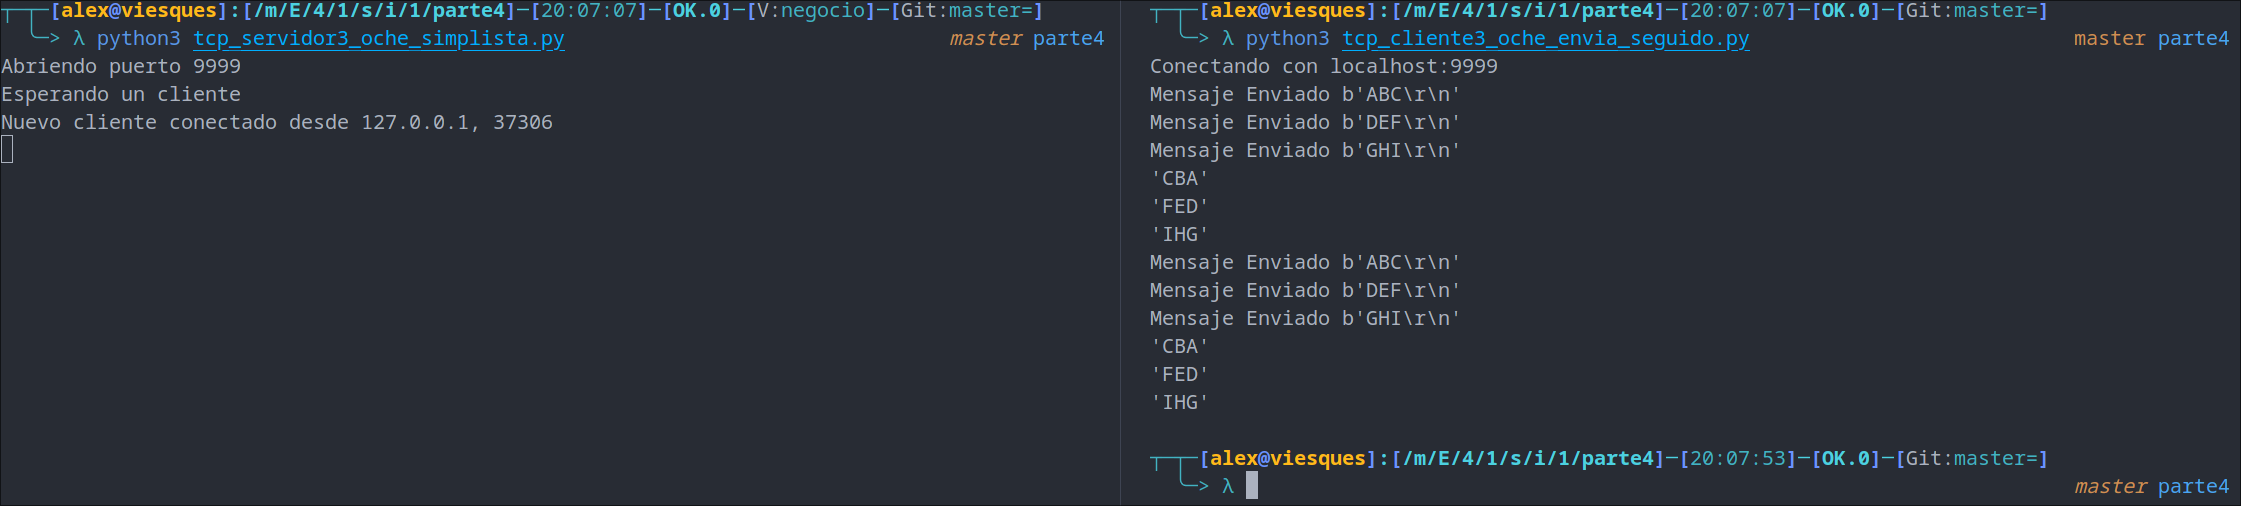
\includegraphics[width=\textwidth]{1/TCP/5.png}
	\captionof{figure}{Envía Seguido}\label{fig:1/7}
\end{minipage}

\begin{notebox}
    Para el desarrollo del servidor,
    se proporcionó en el CV una captura de código
    con el bucle de atención al cliente.

    Este algoritmo no nos funcionó,
    por lo que lo modificamos para que cumpliese su objetivo.

    Si bien en este documento no se muestra todo el código,
    se deja en esta anotación una captura de pantalla del bucle
    de atención al cliente.

	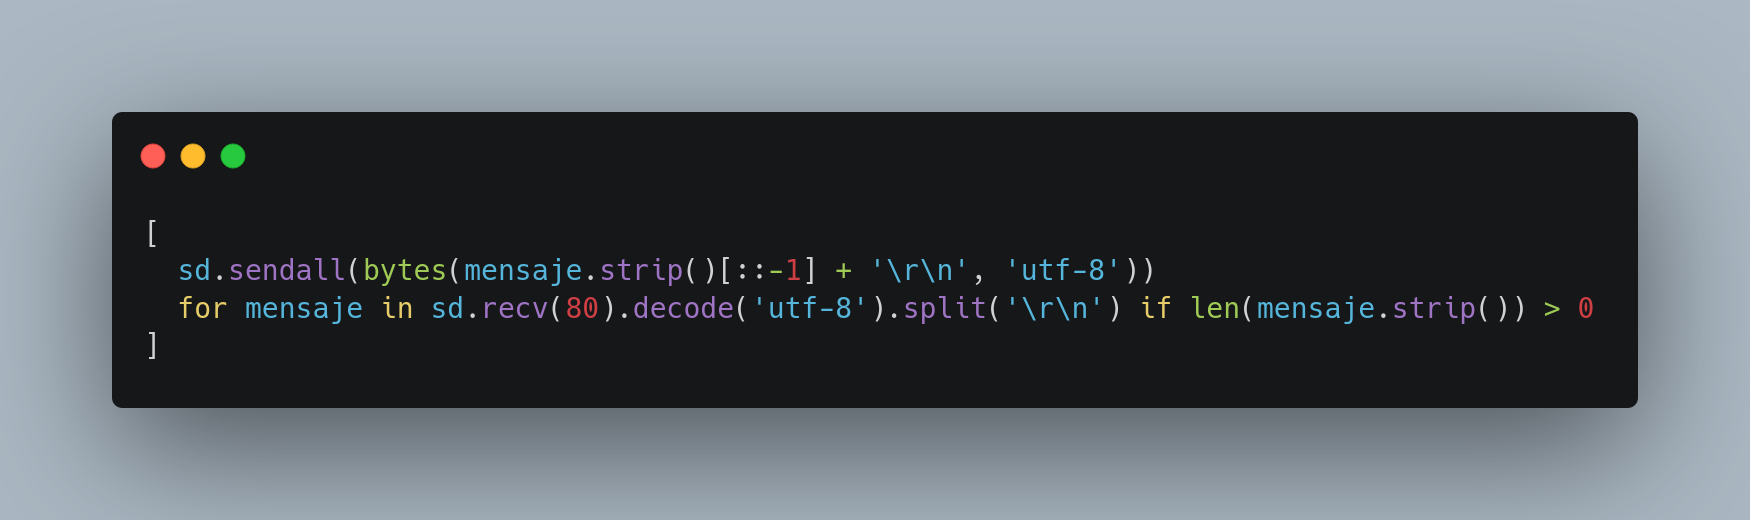
\includegraphics[width=\textwidth]{1/TCP/carbon.png}
\end{notebox}

Posteriormente se añade la función \verb#recibe_mensaje#
para leer datos del socket.
Esta función se implementa en las siguientes versiones del cliente
y servidor.

\begin{minipage}{\linewidth}
	\centering
	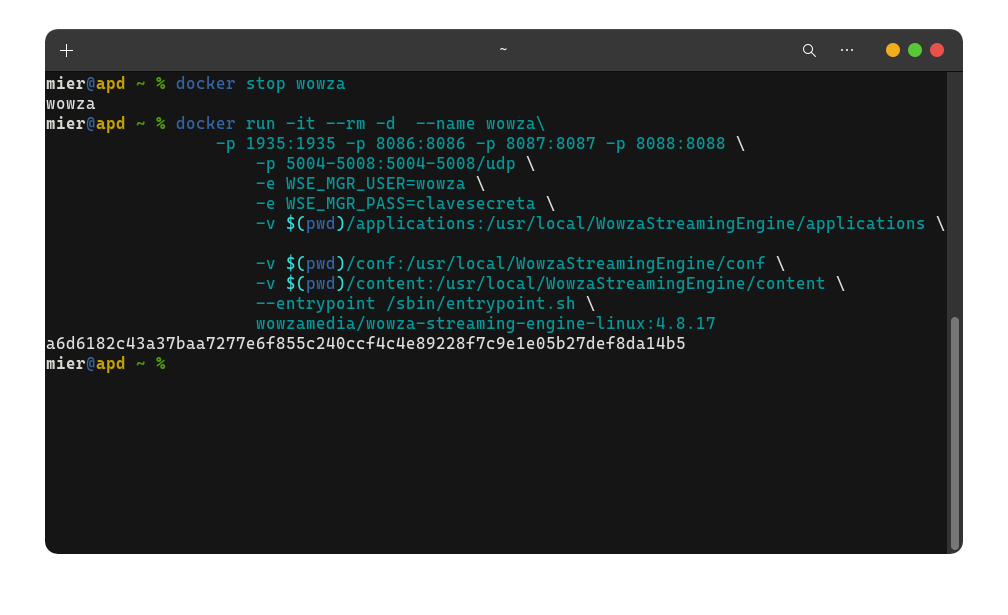
\includegraphics[width=\textwidth]{1/TCP/6.png}
	\captionof{figure}{Servidor y Cliente Mejorados}\label{fig:1/8}
\end{minipage}

Finalmente, se optimiza la función en una nueva llamada \verb#readline#
que no lee los bytes de uno en uno.

\begin{minipage}{\linewidth}
	\centering
	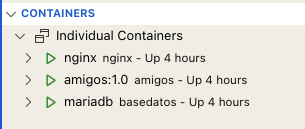
\includegraphics[width=\textwidth]{1/TCP/7.png}
	\captionof{figure}{Readline}\label{fig:1/9}
\end{minipage}

La función \verb#readline# genera un fichero nuevo cada vez que se llama,
por lo tanto, no es posible enviar una cadena con varios saltos
de línea y obtener las líneas independientes con varias llamadas a la
función.

Para poder implementar este funcionamiento,
sería necesario utilizar un iterador que mantuviese el fichero
con \verb#yield# en lugar de \verb#return#.

\subsection{Enviar longitud del mensaje}

Finalmente, la ultima estrategia sería enviar la longitud del mensaje
para que el receptor conozca cuántos bytes debe enviar.

El primer ejemplo envía la longitud del mensaje como un número decimal
al inicio del mensaje.

\begin{minipage}{\linewidth}
	\centering
	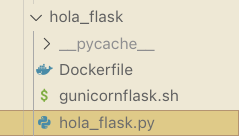
\includegraphics[width=\textwidth]{1/TCP/8.png}
	\captionof{figure}{Cliente y Servidor envían la longitud del mensaje}\label{fig:1/10}
\end{minipage}

El segundo ejemplo envía la longitud del mensaje como un número en binario \\
\verb#big endian# al inicio del mensaje.

\begin{minipage}{\linewidth}
	\centering
	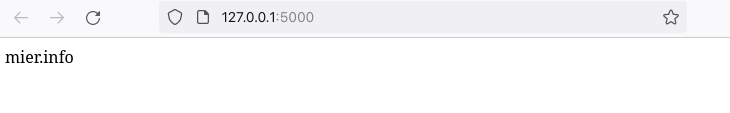
\includegraphics[width=\textwidth]{1/TCP/9.png}
	\captionof{figure}{Resultado de ejecución del ejercicio opcional}\label{fig:1/11}
\end{minipage}

\section{Conclusiones}

El uso de sockets (tanto UDP como TCP) no es nuevo para nosotros, puesto que se han
utilizado previamente en otras asignaturas{ - }por lo tanto, no ha sido una práctica
especialmente difícil ni interesante. Sin embargo, lo que si ha sido interesante es
revisitar las estrategias de TCP para averiguar el fin del mensaje en un lenguaje
diferente y más rápido de escribir que C.

\begin{center}
	\begin{tabular}{|c|c|}
		\hline
		\textbf{Autor} & \textbf{Porcentaje} \\
		\hline
		\hline
		\authorOne & 50\% \\
		\authorTwo & 50\% \\
		\hline
	\end{tabular}
\end{center}
